\documentclass{article}
\usepackage{arxiv}

\usepackage[utf8]{inputenc}
\usepackage[english, russian]{babel}
\usepackage[T1]{fontenc}
\usepackage{url}
\usepackage{booktabs}
\usepackage{amsfonts}
\usepackage{nicefrac}
\usepackage{microtype}
\usepackage{lipsum}
\usepackage{lmodern}
\usepackage{graphicx}
\usepackage{natbib}
\usepackage{doi}



\title{Итеративное улучшение тематической модели с обратной связью от пользователя}

\author{ Горбулев Алексей Ильич \\
	\texttt{gorbulev.ai@phystech.edu} \\
	\And
	Алексеев Василий Антонович \\
	\texttt{vasiliy.alekseyev@phystech.edu} \\
	\And
    Воронцов Константин Вячеславович \\
    \texttt{vokov@forecsys.ru} \\
}
\date{}

\renewcommand{\undertitle}{}
\renewcommand{\shorttitle}{Итеративное улучшение тематической модели с обратной связью от пользователя}

%%% does not show
%%% DeclareMathOperator*{\norm}{norm}

%%% Add PDF metadata to help others organize their library
%%% Once the PDF is generated, you can check the metadata with
%%% $ pdfinfo template.pdf
%%% \hypersetup{
%%% pdftitle={A template for the arxiv style},
%%% pdfsubject={q-bio.NC, q-bio.QM},
%%% pdfauthor={David S.~Hippocampus, Elias D.~Striatum},
%%% pdfkeywords={First keyword, Second keyword, More},
%%% }

\begin{document}
\maketitle

\begin{abstract}
	В работе представлен метод тематического моделирования с использованием обратной связи от пользователя. Обратная связь заключается в определении принадлежности темы, полученной при тематическом моделировании, к одной из трёх категорий: релевантная, нерелевантная, <<мусорная>>. Основная задача состоит в улучшении базовой модели, которое заключается в выделении новых релевантных тем при сохранении выделенных тем и уменьшении числа <<мусорных>> тем. В работе предлагается решение с использованием библиотек тематического моделирования и регуляризаторов сглаживания и декоррелирования. Вычислительный эксперимент проводится на текстовой коллекции, основанной на новостях сайта Lenta.ru.
\end{abstract}

\keywords{Тематическое моделирование \and ARTM \and Обработка естественного языка}

\section{Введение}
Одним из методов анализа текстов, который применяется в том числе в социологических исследованиях \citep{DIMAGGIO2013570} и активно развивается в последнее время \citep{10031921}, является тематическое моделирование.
Тематическая модель помогает оценить вероятность принадлежности текста к каждой из полученных тем.
Именно вероятностное тематическое моделирование использовалось при исследовании распространения информации о пандемии COVID-19 в Хорватии \citep{pandemic2021}, освещения в средствах массовых информации Литвы климатических изменений \citep{climate2021}.

Однако задача построения вероятностной тематической модели имеет бесконечно много решений \citep{bigartm} вследствие некорректной постановки.
С целью ограничения количества решений вводятся регуляризаторы. 
Например, декорреляция способствует улучшению когерентности тем \citep{artm2}, разреживание способствует обнулению части элементов матриц.

В то же время, не все темы могут оказаться \textit{релевантными} в контексте проводимого исследования.
Часть документов, которая по содержанию релевантны, могут быть отнесены как к \textit{нерелевантной} теме, которая дублирует по содержанию релевантную, так и к \textit{<<мусорной>>} теме, которая не имеет отношения к исследованию, что негативно влияет на качество исследования.

Целью данного исследования является построение обновляемой тематической модели с использованием обратной связи от пользователя, найденные релевантные темы которой охватывают в совокупности большую часть коллекции документов.
Пользователь относит каждую из тем к одной из трёх категорий: релевантные, нерелевантные и <<мусорные>> темы. Улучшение модели, которое основывается на пользовательской разметке, способствует сохранению ранее найденных релевантных тем и выделению пользователем новых релевантных тем, а также уменьшению числа <<мусорных тем>>.

Для решения задачи используются в том числе и методы аддитивной регуляризации тематических моделей (ARTM), реализованные в библиотеках с открытым кодом \texttt{BigARTM} и \texttt{TopicNet} \citep{bulatov-etal-2020-topicnet}, которые включают в себя регуляризаторы декоррелирования и сглаживания. Именно подход ARTM способствует оптимизации моделей по сумме нескольких критериев \citep{artm}, что помогает учитывать особенности коллекции текстов и ограничить количество решений задачи тематического моделлирования. В качестве набора текстовых данных используется коллекция, основанная на новостях, опубликованных на сайте Lenta.ru в период с мая по август $2008$ года.

\section{Постановка задачи}

Пусть $D$ — коллекция текстов, $W$ — множество термов.
Среди термов могут быть как ключевые слова, так и словосочетания \citep{artm2}.
Каждый документ $d \in D$ представим в виде последовательности $n_d$ термов $\left( w_1, \dots, w_{n_d} \right)$ из множества $W$ \citep{artm}.
Предполагается конечное множество тем $T$.
Коллекция документов $D$ рассматривается выборка из дискретного распределения $p(w, d, t)$ на конечном множестве $W \times D \times T$ \citep{artm2}.
 Согласно формуле полной вероятности и гипотезе условной независимости, распределение термов в документе $p(w \mid d)$ описывается вероятностной смесью распределений термов в темах $\varphi_{wt} = p(w \mid t)$ с весами $\theta_{td} = p (t \mid d)$ следующим образом: \citep{bigartm}
 \begin{equation}
      p(w \mid d) = \sum \limits_{t \in T} p(w \mid t, d) p(t \mid d) = \sum \limits_{t \in T} p (w \mid t) p (t \mid d) = \sum \limits_{t \in T} \varphi_{wt} \theta_{td}
 \end{equation}
 Задача тематического моделирования состоит в нахождении по коллекции документов $D$ параметров $\varphi_{wt}$ и $\theta_{td}$, приближающих частотные оценки условных вероятностей $\widehat{p} (w \mid d)$.
 Так как $|T|$ обычно намного меньше, чем $|W|$ и $|D|$, то находится низкоранговое стохастическое матричное разложение \citep{artm2}
 \begin{equation}
     F \approx \Phi \Theta
 \end{equation}
 где $F = {(\widehat{p}_{wd})}_{|W| \times |D|}$ — матрица частот терм в документах, $\Phi = {(\varphi_{wt})}_{|W| \times |T|}$ — матрица термов тем, $\Theta = {(\theta_{td})}_{|T| \times |D|}$ — матрица тем документов.

Предполагается $T^i$ — множество тем на итерации $i \in \mathbb{N}$,  $T_+^i \subset T^i$ — подмножество релевантных тем с точки зрения пользователя, $T_0^i \subset T^i$ — подмножество нерелевантных тем с точки зрения пользователя, $T_-^i \subset T_i$ — подмножество <<мусорных>> тем с точки зрения пользователя, при этом $T^i = T_+^i \sqcup T_0^i \sqcup T_-^i$, $M_i$ — состояние модели на итерации $i$.
Тогда итеративное улучшение модели $M_i$ состоит в построении модели $M_{i + 1}$, такой, чтобы множество тем $T_{i + 1}$ удовлетворяло следующим требованиям:

$$T_i^1 \subset T_{i + 1}^1, \ \left| T_{i + 1}^3 \right| \leq \left| T_i^3 \right|$$

\section{Метод}

Предполагается при обучении новой модели $M_{i + 1}$ использовать аддитивную регуляризацию тематических моделей (ARTM) и выполнить следующее:

\begin{enumerate}
    \item Использовать альтернативное значение параметра, отвечающего за генерацию случайного начального приближения;
    \item При инициализации матрицы $\Phi$ зафиксировать столбцы, соответствующие релевантным темам $T_+^i$, используя регуляризатор сглаживания, общий вид формулы которого \citep{SukVor19}
    \begin{equation}
        R (\Phi, \Theta) = \beta_0 \sum \limits_{t \in T} \sum \limits_{w \in W} \beta_{wt} \ln \varphi_{wt} + \alpha_0 \sum \limits_{d \in D} \sum \limits_{t \in T} \alpha_{td} \ln \theta_{td} \to \max \limits_{\Phi, \Theta}
    \end{equation}
    Коэффициент $\tau$, соответствующий данному регуляризатору, должен быть достаточно большим для фиксации. В вычислительном эксперименте рассматривается значение $\tau$, равное ${10}^9$. 
    При использовании другого значения параметра, ответственного за генерацию случайного начального приближения, нерелевантные темы могут не сохраниться, и может увеличиться число <<мусорных>> тем.
    Вследствие этого предлагается также зафиксировать столбцы, соответствующие нерелевантным темам $T_0^i$, так как тема может не полностью пересекаться с соответствующей ей релевантной.
    \item Чтобы способствовать выявлению новых релевантных тем, предлагается использовать регуляризатор декоррелирования, используя матрицу $\widetilde{\Phi}$ из модели $M_i$:
    \begin{equation}
        R(\Phi) = -\tau \sum \limits_{t \in T_+} \sum \limits_{s \in T_-} \sum \limits_{w \in W} \varphi_{wt} \widetilde{\varphi}_{ws} \to \max
    \end{equation}
    \begin{equation}
        R(\Phi) = -\tau \sum \limits_{t \in T_+ \\ s \in T_-} \left\langle \varphi_t, \widetilde{\varphi}_s \right\rangle \to \max
    \end{equation}
    \begin{equation}
        R(\Phi) = -\tau \sum \limits_{t \in T_+} \left\langle \varphi_t, \sum \limits_{s \in T_-} \widetilde{\varphi}_s \right\rangle \to \max
    \end{equation}
    \begin{equation}
        \frac{\partial R}{\partial \varphi_{wt}} = -\tau [t \in T_+] \sum \limits_{s \in T_-} \widetilde{\varphi}_{ws}
    \end{equation}
    \begin{equation}
        \varphi_{wt} = {norm}_{w \in W} \left(n_{wt} - \tau \varphi_{wt} [t \in T_+] \sum \limits_{s \in T_-} \widetilde{\varphi}_{ws}\right)
    \end{equation}
\end{enumerate}

В качестве внешнего критерия предлагается использовать количество тем в $T_+$, $T_0$ и $T_-$.
Чем больше тем в $T_+$ и меньше тем в $T_i$, тем лучше.

В качестве внутреннего критерия предлагается использовать следующие метрики:

\begin{enumerate}
    \item Перплексия \citep{bigartm}
    \begin{equation}
        \mathcal{P}_m (D; p) = \exp \left( - \frac{1}{n_m} \sum \limits_{d \in D} \sum \limits_{w \in W^m} n_{dw} \ln p (w \mid d) \right)
    \end{equation}
    \item Разреженность матрицы $\Phi$
    \item Средняя контрастность тем \citep{bigartm}, где контрастность темы определяется как
    \begin{equation}
        {con}_t = \frac{1}{|W_t|} \sum \limits_{w \in W_t} p(t \mid w)
    \end{equation}
    \begin{equation}
        W_t = \{ w \in W \mid \varphi_{wt} > \frac{1}{|W|} \}
    \end{equation}
\end{enumerate}

\section{Вычислительный эксперимент}

\href{https://github.com/intsystems/2023-Project-131/blob/master/code/Experiment_Tuning_Last.ipynb}{Вычислительный эксперимент} был произведён на языке Python с использованием библиотек с открытым исходным кодом BigARTM и TopicNet.

\subsection{Описание данных}

Для обучения тематических моделей использовалась \href{https://disk.yandex.ru/d/DAdhmVB2eFkdBQ}{коллекция новостей}, опубликованных на сайте Lenta.ru с $1$ мая по $31$ августа $2008$ года.
Каждая из $16449$ новостей распределена по одной из $11$ макротем:

\begin{enumerate}
    \item <<Бывший СССР>>
    \item <<Дом>>
    \item <<Из жизни>>
    \item <<Интернет и СМИ>>
    \item <<Культура>>
    \item <<Мир>>
    \item <<Наука и техника>>
    \item <<Россия>>
    \item <<Силовые структуры>>
    \item <<Спорт>>
    \item <<Экономика>> 
\end{enumerate}

Новости, относящиеся к одной из макротем, могут быть отнесены как к релевантной, так и к <<мусорной>> теме. В связи с этим предлагается в качестве параметра, отвечающее за количество предметных тем $|T|$, использовать значение, равное $50$.

\subsection{Предобработка}

Заголовки и тексты каждой новости были разбиты на токены, которые представляют собой отдельные слова.
Далее посредством морфологического анализатора \texttt{pymorphy2} \citep{pymorphy2} была произведена лемматизация токенов, которые не вошли в список стоп-слов.
Из двух подряд идущих лемматизированных токенов были составлены биграммы. Далее по метрике PMI (pointwise mutual information, поточечная взаимная информация) были отобраны $10 000$ биграмм, которые характеризуют каждый документ из коллекции. Далее произошло преобразование в формат, совместимый с Vowpal Wabbit, чтобы обеспечить работу с TopicNet.

Суммарно предобработка прошла за $11$ минут $14$ секунд.

\subsection{Базовая модель}

В качестве базовой модели $M_0$ используется тематическая модель, не имеющая регуляризаторов, действующих на столбцы матрицы $\Phi$, соответствующих специальным темам, и имеющая регуляризаторы сглаживания, действующие на столбцы матриц $\Phi$ и $\Theta$, соответствующие фоновой теме, имеющие коэффициенты, равные $0$.
Используются две модальности:
\begin{enumerate}
    \item По лемматизированным токенам (\texttt{@lemmatized}), коэффициент $1.0$;
    \item По биграммам (\texttt{@bigram}), коэффициент $0.8$.
\end{enumerate}
В качестве значения параметра \texttt{seed}, отвечающего за генерацию случайного начального приближения, используется $21$.
Обучение модели $M_0$ происходит в течение $50$ итераций.

\subsection{Создание новой модели}

Пусть известна пользовательская разметка на основе тематической модели $M_{i - 1}$, а также параметры модели $M_{i - 1}$.
Создание модели $M_i$ происходит с соблюдением следующих правил:
\begin{enumerate}
    \item Значение параметра \texttt{seed} увеличивается на $21$;
    \item С помощью регуляризатора сглаживания происходит фиксация тем из $T_+^{i - 1}$ и $T_0^{i - 1}$;
    \item Создаётся регуляризатор декоррелирования $(4)$ для тем из $T_+^{i - 1}$ и $T_-^{i - 1}$;
    \item Остальные параметры сохраняются.
\end{enumerate}
Одним из недостатков тематического моделирования в целом является неполнота моделей и отсутствие однозначного решения задачи \citep{bigartm}, а также зависимость от случайности.
Одним из способов избавления от случайности является использование различных значений параметров \texttt{seed} при обучении разных версий моделей.

\subsection{Результаты}

После обучения базовой модели $M_0$ пользователем было выделено $5$ релевантных тем:

\begin{enumerate}
    \item $12$ (Дмитрий Медведев и его международные контакты)
    \item $21$ (события на Кавказе в августе 2008 года)
    \item $29$ (Украина, политика и ситуация по переговорам по газовой сделке)
    \item $30$ (президентские выборы в США, 2008)
    \item $35$ (Путин в качестве премьер-министра)
\end{enumerate}

Была выделена $1$ нерелевантная тема $31$, в большинстве своём дублирующая тему $21$.
Была создана модель $M_1$, содержащийся в ней регуляризатор фиксации тем помог сохранить ранее найденные релевантные темы.
Кроме того, были выделены ещё $2$ релевантные темы:
\begin{enumerate}
    \item $14$ (санкции США против Ирана)
    \item $15$ (выборы, ситуация в Зимбабве)
\end{enumerate}
После обучения ещё одной новой модели $M_2$ выяснилось, что темы из $T_+^1$ были сохранены, также удалось выделить релевантную тему $46$ о Гаагском трибунале.
После обучения $M_3$ разметка тем по трём категориям не изменилась по сравнению с $M_2$.

\begin{table}[]
    \centering
    \begin{tabular}{c|c|c|c|}
        Модель & $|T_+|$ & $|T_0|$ & $|T_-|$ \\
        \hline
        $M_0$ & $5$ & $1$ & $44$ \\
        $M_1$ & $7$ & $1$ & $42$ \\
        $M_2$ & $8$ & $1$ & $41$ \\
        $M_3$ & $8$ & $1$ & $41$
    \end{tabular}
    \caption{Данные по группам по пользовательской разметке}
    \label{tab:my_label}
\end{table}

По обоим модальностям модели $M_1$ и $M_2$ обладают меньшей перплексией, чем $M_0$, что обычно происходит при использовании регуляризаторов. \citep{artm2}
В то же время, после $50$ итераций обучения модель $M_3$ обладает перплексией, схожей с перплексией модели $M_0$.

\begin{figure}[h]
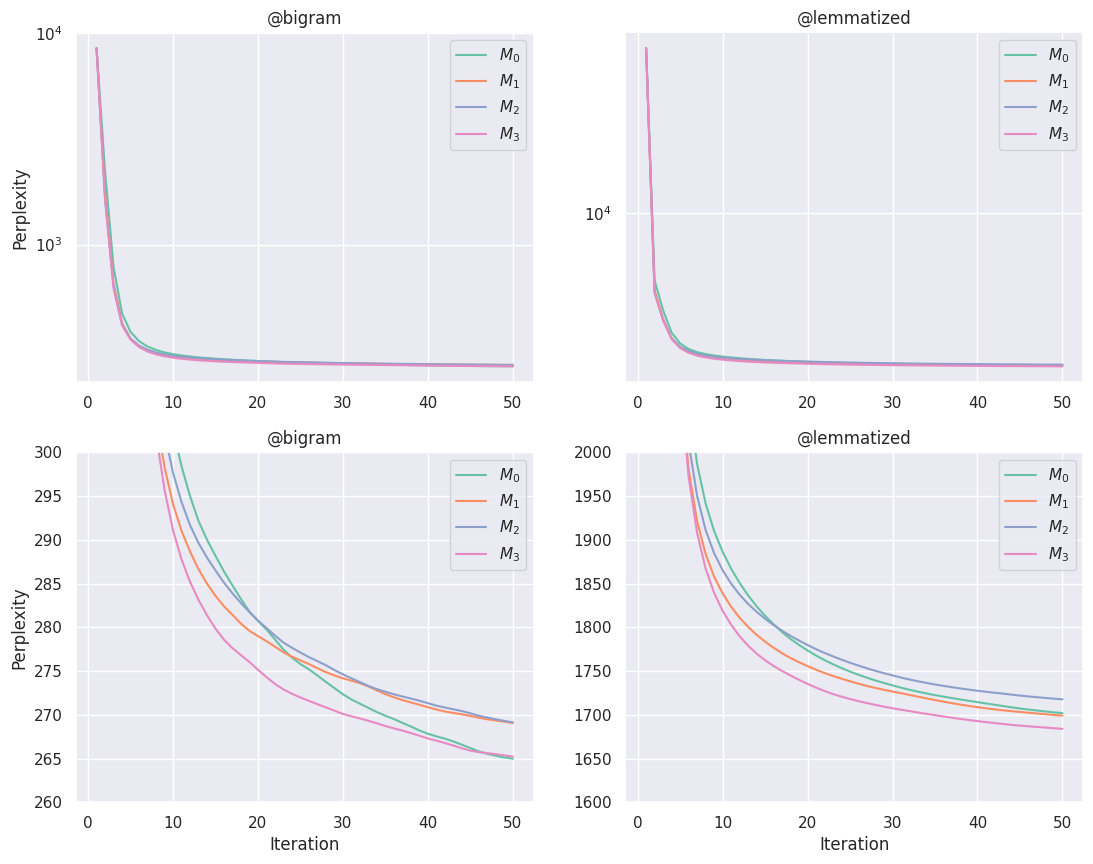
\includegraphics[width=8cm]{figures/perplexity_v3.png}
\centering
\caption{Перплексия}
\end{figure}

Различия по разреженности матрицы $\Phi$ крайне незначительны от модели к модели и находятся в пределах статистической погрешности.

\begin{figure}[h]
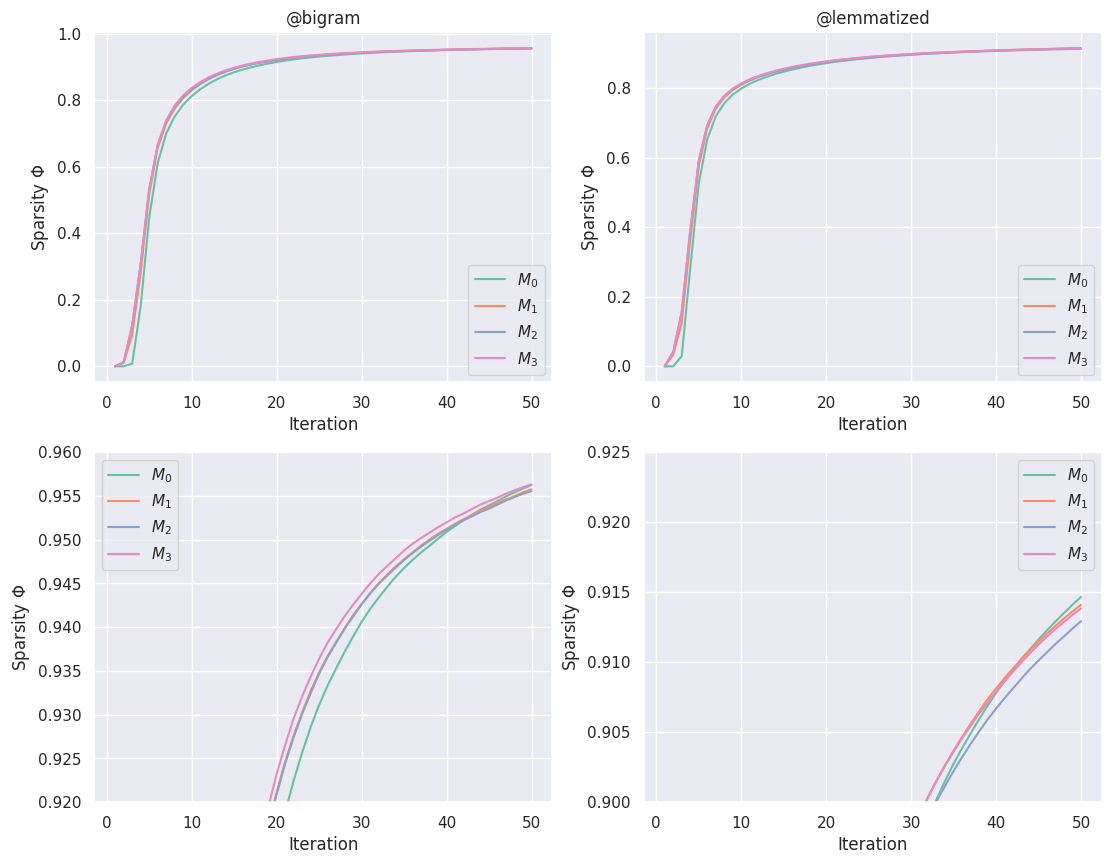
\includegraphics[width=8cm]{figures/sparsity_v3.png}
\centering
\caption{Разреженность матрицы $\Theta$}
\end{figure}

По средней контрастности тем модель $M_3$ показывает схожие результаты с $M_0$, которые являются сравнительно лучшими по модальности биграмм.
С точки зрения модальности лемматизированных слов, модель $M_0$ обладает более высокой средней контрастностью тем, чем остальные.
В то же время, различия являются несущественными.

\begin{figure}[h]
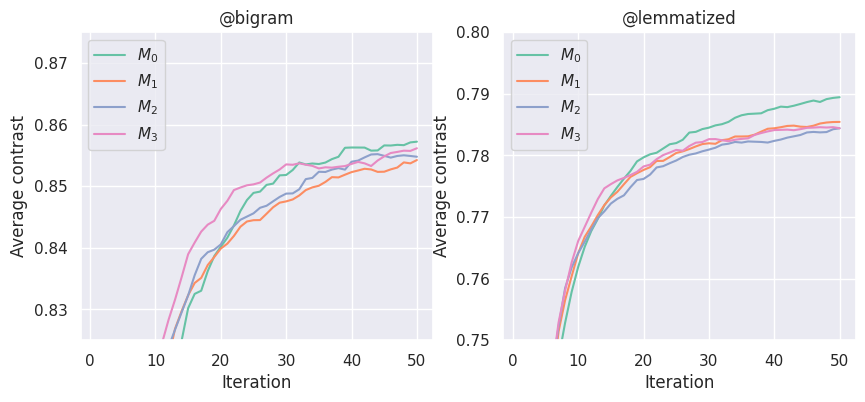
\includegraphics[width=12cm]
{figures/avg_contrast_v3.png}
\centering
\caption{Средняя контрастность тем}
\end{figure}

\section{Заключение}

В данной работе был предложен метод итеративного улучшения тематической модели с помощью фиксации релевантных тем через регуляризатор сглаживания и декоррелирования тем.
Вычислительный эксперимент показал, что регуляризатор сглаживания, действующий на столбцы матрицы $\Phi$, соответствующий релевантным темам, действительно способствует сохранению тем.
Кроме того, удалось добиться увеличения количества релевантных тем.
В дальнейшем планируется исследование не только на коллекциях новостей, но и на коллекциях специализированных текстов, чтобы проверить универсальность предложенного метода.

\bibliographystyle{plain}
\bibliography{Gorbulev2023TopicModels}

\end{document}